\documentclass[12pt,a4paper]{report}

\usepackage[utf8]{inputenc}
\usepackage[T5]{fontenc}
\usepackage{mathptmx}
\usepackage{amsmath}
\usepackage{graphicx}
\usepackage{float}
\usepackage{tikz}
\usetikzlibrary{calc,positioning}

\graphicspath{{docs/}{docs/figures/}{figures/}}

\begin{document}

% ====== TITLE PAGE ======
\begin{titlepage}
\centering
\vspace*{2cm}

{\Large \textbf{SPEC DỰ ÁN 1}\par}
\vspace{0.5cm}
{\LARGE \textbf{Khối điều khiển nhiệt ẩm công suất cao (Peltier 110W)}\par}

\vspace{1.5cm}
{\large Tài liệu đặc tả kỹ thuật (Standalone)\par}

\vfill
{\large \today\par}
\end{titlepage}

\tableofcontents
\clearpage

% ====== MAIN CONTENT ======
\chapter{Dự án 1 --- Khối điều khiển nhiệt ẩm công suất cao (Peltier 110W)}

\section{Mục tiêu và phạm vi}
Mục tiêu vận hành của khối là duy trì điều kiện môi trường trong buồng đo ở mức nhiệt độ $T \in [20, 25]\,^\circ$C và độ ẩm $H \in [60, 65]\%RH$. Phương pháp điều khiển là làm lạnh để ngưng tụ hút ẩm (Peltier) kết hợp quạt/tản nhiệt, điều khiển theo luật On--Off có hysteresis và giới hạn thời gian bật/tắt tối thiểu để tránh đóng/ngắt liên tục.

Phạm vi điều khiển tập trung vào đóng/ngắt nguồn DC 12V cấp cho Peltier bằng MOSFET (ưu tiên module có opto cách ly).

\section{Kiến trúc hệ thống}
\subsection{Sơ đồ khối và luồng tín hiệu}
\begin{figure}[H]
\centering
\begin{tikzpicture}[
  node distance=12mm,
  block/.style={draw, rounded corners, align=center, minimum width=28mm, minimum height=10mm},
  small/.style={draw, rounded corners, align=center, minimum width=22mm, minimum height=8mm},
  arrow/.style={->, thick}
]
  \node[block] (sht) {SHT35\\(I\textsuperscript{2}C)};
  \node[block, right=18mm of sht] (esp) {ESP32\\(Control)};
  \node[block, right=18mm of esp] (mos) {MOSFET\\Power Stage\\(12V, $>10$A)};
  \node[block, right=18mm of mos] (pel) {Peltier 110W\\+ Heatsink\\+ Fan};

  \node[small, below=10mm of esp] (cfg) {Setpoint\\Hysteresis\\Min ON/OFF};
  \node[small, above=10mm of mos] (prot) {Bảo vệ\\Quá nhiệt\\(tuỳ chọn)};

  \draw[arrow] (sht) -- node[above]{T/H} (esp);
  \draw[arrow] (esp) -- node[above]{GPIO (ON/OFF)} (mos);
  \draw[arrow] (mos) -- node[above]{12V} (pel);
  \draw[arrow] (cfg) -- (esp);
  \draw[arrow] (prot) -- (mos);
\end{tikzpicture}
\caption{Sơ đồ khối dự án 1: điều khiển Peltier hút ẩm công suất cao}
\label{fig:p1_block}
\end{figure}

\subsection{Ảnh minh hoạ phần cứng chính}
\begin{figure}[H]
\centering
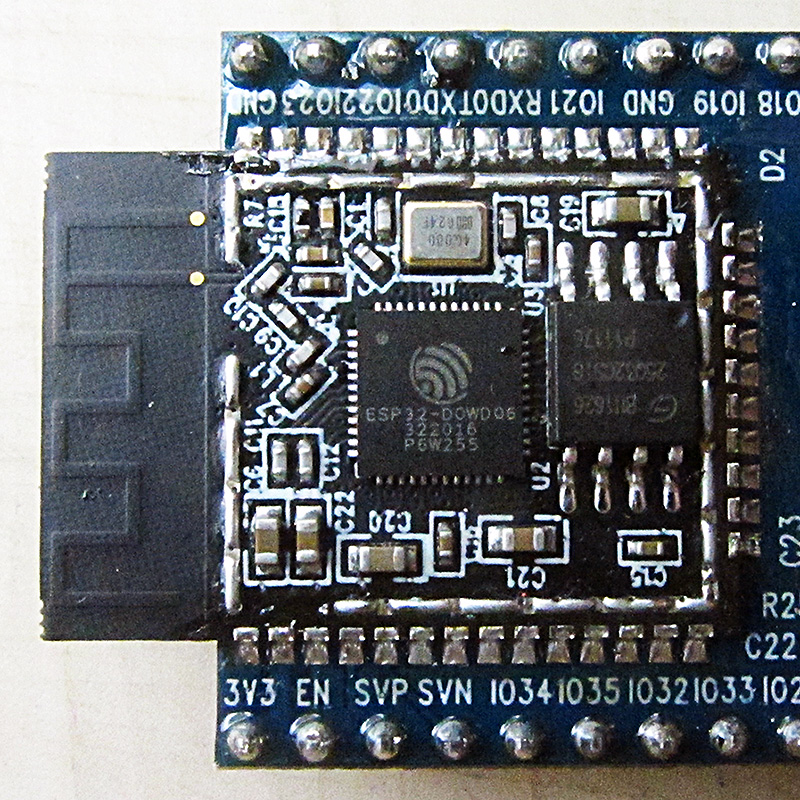
\includegraphics[width=0.6\textwidth]{figures/p1_esp32_overview.jpg}
\caption{Cận cảnh module ESP32 DevKit được sử dụng làm khối điều khiển trung tâm cho hệ thống điều khiển nhiệt ẩm.}
\label{fig:p1_esp32_overview}
\end{figure}

\begin{figure}[H]
\centering
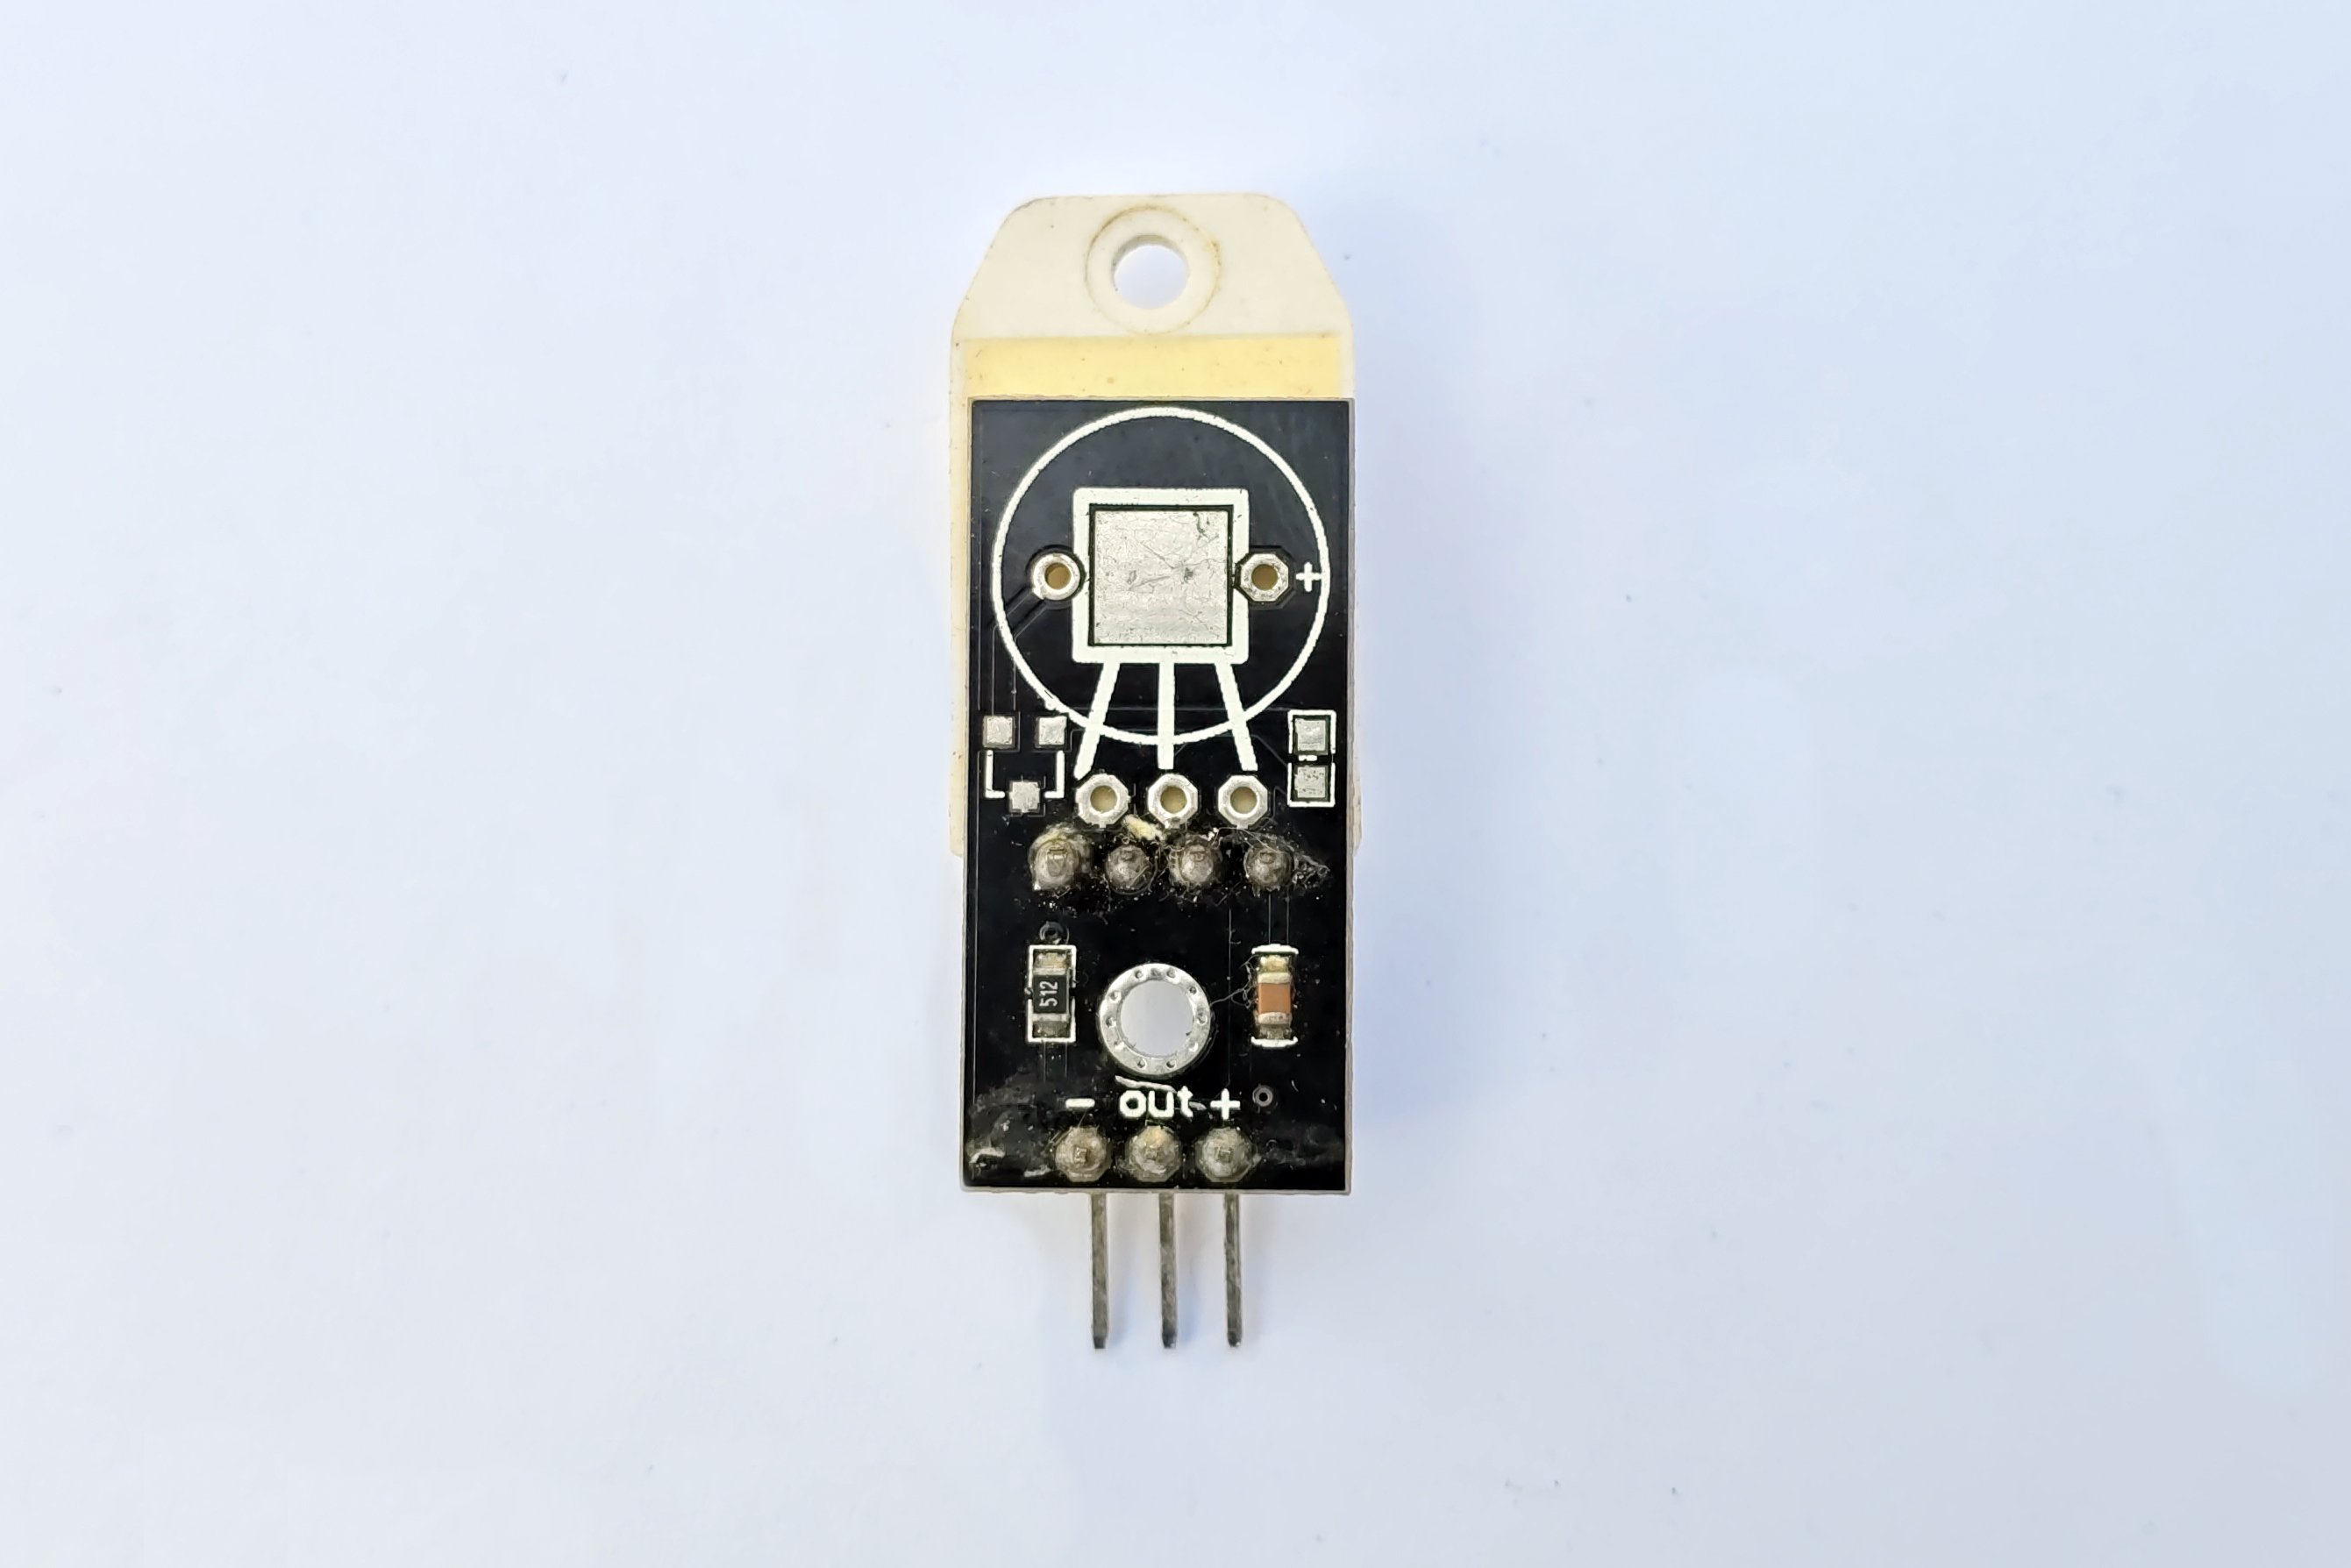
\includegraphics[width=0.45\textwidth]{figures/p1_env_sensor_module.jpg}
\caption{Module cảm biến môi trường dạng breakout ba chân, dùng làm minh hoạ cho cảm biến nhiệt độ--độ ẩm đặt trong buồng đo.}
\label{fig:p1_env_sensor}
\end{figure}

\section{I/O và giao tiếp}
\subsection{Bảng I/O tối thiểu}
\begin{table}[H]
\centering
\caption{Bảng I/O tối thiểu --- Dự án 1}
\begin{tabular}{|p{3.2cm}|p{2.2cm}|p{3.4cm}|p{6.2cm}|}
\hline
\textbf{Khối} & \textbf{Loại} & \textbf{Tín hiệu} & \textbf{Yêu cầu/ghi chú}\\
\hline
SHT35 & I\textsuperscript{2}C & SDA/SCL & 3.3V logic; pull-up theo module; đọc 1--2 Hz\\
\hline
ESP32 $\rightarrow$ MOSFET & Digital output & GPIO\_PEL\_EN & Điều khiển ON/OFF; ưu tiên module MOSFET có opto cách ly\\
\hline
Nguồn 12V & Power & 12V\_IN & Dòng cực đại hệ Peltier $\approx 10$A; khuyến nghị nguồn 12V--20A\\
\hline
Quạt tản nhiệt & Power/Control & FAN\_12V & Có thể chạy liên tục khi Peltier hoạt động; hoặc thêm MOSFET điều khiển riêng\\
\hline
(Tuỳ chọn) NTC/DS18B20 & Sensor & T\_HOT & Bảo vệ quá nhiệt mặt nóng; ngắt Peltier khi vượt ngưỡng\\
\hline
UART log & Debug & TX/RX & Log: $T/H$, trạng thái Peltier, lỗi cảm biến\\
\hline
\end{tabular}
\end{table}

\section{Yêu cầu cơ khí và kích thước}
Để triển khai ổn định và lắp đặt dễ dàng, cần bổ sung các ràng buộc cơ khí sau (đề xuất, có thể cập nhật theo hộp/khung thực tế):
\begin{itemize}
  \item \textbf{Khu vực lắp Peltier + heatsink}: cần mặt phẳng tiếp xúc tốt, có lực ép đều, sử dụng keo tản nhiệt; bố trí đường thoát nước ngưng tụ (nếu có).
  \item \textbf{Không gian tản nhiệt}: đảm bảo khe thoáng khí cho quạt (tối thiểu 10--15mm trước/sau cánh quạt), tránh recirculation khí nóng.
  \item \textbf{Dây nguồn tải}: chọn tiết diện phù hợp dòng 10A; khuyến nghị dùng terminal bắt vít chắc chắn, hạn chế mối nối lỏng gây nóng.
  \item \textbf{Cách ly nhiễu}: tách đường tín hiệu I\textsuperscript{2}C và dây công suất; đi mass kiểu ``star ground'' nếu không cách ly quang.
\end{itemize}

\section{Thuật toán điều khiển (On--Off + hysteresis)}
\textbf{Luật bật/tắt}: bật làm lạnh/hút ẩm khi $(T > 25^\circ C)$ \textbf{hoặc} $(H > 65\%)$; tắt khi $(T < 20^\circ C)$ \textbf{và} $(H < 60\%)$.

Để tránh dao động:
\begin{itemize}
  \item \textbf{Lọc số}: trung bình trượt 5--10 mẫu cho $T/H$ (chu kỳ đọc 0.5--2 Hz).
  \item \textbf{Min ON/OFF time}: 10--30 giây cho mỗi lần bật/tắt.
  \item \textbf{Bảo vệ quá nhiệt (tuỳ chọn)}: tắt Peltier khi $T_{hot} > T_{limit}$ và chỉ cho phép bật lại khi giảm dưới ngưỡng an toàn.
\end{itemize}

\begin{figure}[H]
\centering
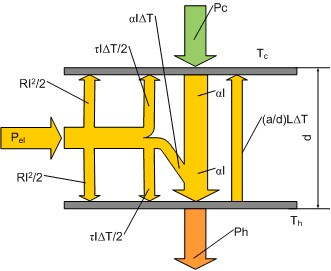
\includegraphics[width=0.5\textwidth]{figures/p1_peltier_principle.jpg}
\caption{Sơ đồ nguyên lý truyền nhiệt trong khối Peltier: công suất điện cấp vào, dòng nhiệt đi từ mặt lạnh sang mặt nóng và các thành phần tổn hao.}
\label{fig:p1_peltier_principle}
\end{figure}

\section{Tích hợp hệ thống (kết nối mesh WiFi)}
Trong hệ thống tổng thể, node Peltier của dự án 1 được triển khai như một node con trong mạng WiFi mesh ESP32 (dự án 3). Node này gia nhập mesh, nhận lệnh điều khiển ngưỡng $T/H$ và trạng thái bật/tắt từ root node, đồng thời gửi telemetry nhiệt độ--độ ẩm và trạng thái Peltier về gateway để HMI và backend giám sát.

\end{document}